\documentclass[12pt]{article}
\usepackage{graphicx} % Required for inserting images
\usepackage{amsmath,amssymb,amsthm,amsfonts}
\usepackage{xcolor}
\usepackage{tasks}
%\usepackage{enumitem}
\usepackage[margin=2cm]{geometry}
\usepackage{tkz-euclide}

\usepackage[utf8]{inputenc}
\usepackage[T1]{fontenc}
\usepackage{amsmath}
\usepackage{amsfonts}
\usepackage{amssymb}
\usepackage[version=4]{mhchem}
\usepackage{stmaryrd}
\usepackage{enumerate}
\usepackage{multicol}
\usepackage{xcolor}
\usepackage{graphicx}
\usepackage{ulem}
\usepackage{cancel}
\usepackage{tikz}
\usepackage{tkz-euclide}
\usepackage[finnish]{babel}

%\usepackage[style=alphabetic,]{biblatex}

%\usepackage[margin=2cm]{geometry}

\newcommand{\brac}[1]{\left(#1\right)}
\newcommand{\sqbrac}[1]{\left[#1\right]}
\newcommand{\set}[1]{\left\{#1\right\}}

\newcommand{\dd}[0]{\mathrm{d}}
\newcommand{\dx}[0]{\mathrm{d}x}

\newcommand{\hatu}{\hat{u}}
\newcommand{\hatv}{\hat{v}}
\newcommand{\hatw}{\hat{w}}
\newcommand{\hatn}{\hat{n}}

\newcommand{\vu}{\overline{u}}
\newcommand{\vv}{\overline{v}}
\newcommand{\vw}{\overline{w}}
\newcommand{\vp}{\overline{p}}
\newcommand{\vn}{\overline{n}}

\newcommand{\va}{\overline{a}}
\newcommand{\vb}{\overline{b}}
\newcommand{\vc}{\overline{c}}
\newcommand{\vd}{\overline{d}}


\newcommand{\vi}{\hat{\imath}}
\newcommand{\vj}{\hat{\jmath}}
\newcommand{\vk}{\hat{k}}

\newcommand{\ratkaisu}[1]{\hfill{\color{blue}\quad\textrm{Ratkaisu: } #1}}

\newcommand{\ratkaisuu}[1]{{\color{blue}\textrm{Ratkaisu: } #1}}

\newcommand{\kaava}[1]{{\color{green!50!black}#1}}

%\renewcommand{\ratkaisu}[1]{}
%\renewcommand{\ratkaisuu}[1]{}
%\renewcommand{\kaava}[1]{}

\newcommand{\vihje}[1]{{\color{red}Vihje. #1}}
\newcommand{\extra}[0]{\textbf{Extra.}~}

\title{OAMK}
\author{Juha-Matti Huusko}
\date{August 2023}

\renewcommand{\ratkaisu}[1]{{\color{blue}\quad\textrm{Ratkaisu: } #1}}

%\renewcommand{\ratkaisu}[1]{}

\begin{document}
\thispagestyle{empty}

\section*{Matematiikan koe}
\subsubsection*{Matematiikan perusteet tietotekniikassa 2, IN00EH21-3002}

Laske kaikki kuusi tehtävää.

\begin{enumerate}
\item Laske $f'(x)$, kun
\begin{enumerate}
\item $f(x)=4x^5-\sqrt{x}+\frac{1}{x^2}$
\ratkaisu{$20x^4-\frac{1}{2\sqrt{x}}-\frac{2}{x^3}$}
\item $f(x)=3\sin(2x)-7e^{x^3}$
\ratkaisu{$6\cos(2x)-21x^3e^{x^3}$}
\item $f(x)=5x^2\ln(x)$
\ratkaisu{$10x\ln(x)+5x$}
\end{enumerate}
\item Laske funktion $f(x)=4\sin(x)-\cos(2x)$ hetkellinen muutosnopeus pisteessä $x=\frac{\pi}{2}$.
\ratkaisu{Derivaattafunktio on $f'(x)=4\cos(x)+2\sin(2x)$. Sen kysytty arvo on $f'(\frac{\pi}{2})=4\cdot 0+2\cdot 0=0$, koska $\cos(\pi/2)=0$ ja $\sin(2\pi/2)=\sin(\pi)=0$}
\item Millä muuttujan \(x>0\) arvolla funktio \(f(x)=x^3e^{-7x}\) saa maksimiarvonsa?
\ratkaisu{Funktion derivaatta on tulon derivoinnilla
$$
f'(x)=3x^2e^{-7x}+x^3e^{-7x}\cdot (-7)
=x^2e^{-7x}(3-7x)=0,
$$
kun $x=\frac37$.
}
\item Laske
\begin{enumerate}
\item $\int 4x+\sqrt{x}dx$
\ratkaisu{$2x^2+\frac23 x^{\frac32}+C$}
\item $\int \cos(2x)dx$
\ratkaisu{$\frac12\sin(2x)+C$}
\item $\int_2^3 e^{-x}+1dx$
\ratkaisu{Funktion $f(x)=e^{-x}+1$ eräs integraalifunktio on $F(x)=-e^{-x}+x$. Sijoitukseksi saadaan
$$
F(3)-F(2)=-e^{-3}+3-(-e^{-2}+2)=e^{-2}-e^{-3}+1.
$$}
\end{enumerate}

\item Integraalille $\int_0^\pi \sin(x)dx$ voidaan laskea arvio vasemman päätepisteen menetelmällä. Jaetaan integroimisväli neljään osaan. Piirrä kuva vasemman päätepisteen menetelmän toiminnasta. (Kuva riittää, ei tarvitse laskea mitään.)

\ratkaisu{Piirretään}
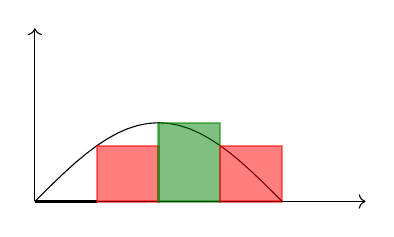
\begin{tikzpicture}
%\draw (0,0) grid (4,2);
\draw[->] (0,0)--(4.2,0);
\draw[->] (0,0)--(0,2.2);
\draw[domain=0:3.14] plot (\x,{sin(\x r)});
\filldraw[thick,black] (0,0)--(0.785,0);
\filldraw[thick,red,opacity=0.5] (0.785,0)--(1.57,0)--(1.57,0.707)--(0.785,0.707)--cycle;
\filldraw[thick,green!50!black,opacity=0.5] (1.57,0)--(2.355,0)--(2.355,1)--(1.57,1)--cycle;
\filldraw[thick,red,opacity=0.5] (2.355,0)--(3.14,0)--(3.14,0.707)--(2.355,0.707)--cycle;
\end{tikzpicture}


\item Tarkastellaan funktiota $f(x)=x^2$. Piirrä funktion kuvaaja. (Luonnos riittää.)
\begin{enumerate}
\item Piirrä kuvaajalle tangenttisuora kohtaan $x=2$. Laske tangenttisuoran kulmakerroin.
\ratkaisu{Funktion derivaattafunktio on $f'(x)=2x$. Kulmakerroin on $f'(2)=2\cdot 2=4$.}
\item Laske $\int_0^2 f(x)dx$. Varjosta pinta-ala kuvaan.
\ratkaisu{Saadaan
$$
\int_0^2x^2dx=\bigg/_0^2 \frac13x^3=\frac13(2^3-0^3)=\frac83.
$$}
\end{enumerate}

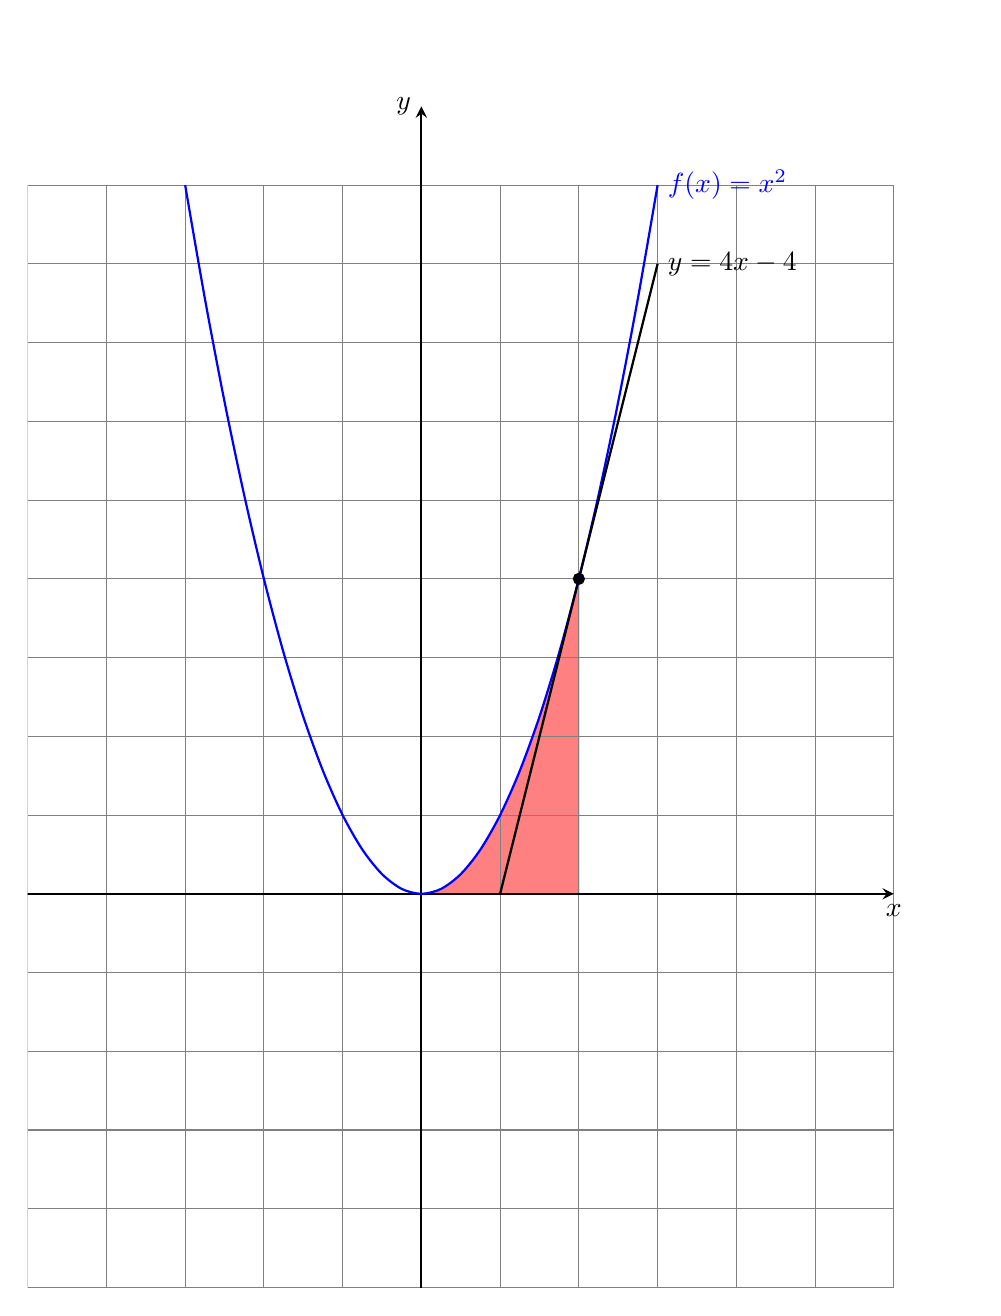
\begin{tikzpicture}[>=stealth]
\path[clip] (-5,-5) rectangle (7,11);
\filldraw[color=red!50!white, smooth, domain=0:2]   plot (\x,\x*\x) -- (2,0)--(0,0)--cycle;
\draw[gray] (-8.9,-8.9) grid (6,9);
\draw[->,thick] (-10,0) -- (6,0) node[below]{$x$};
\draw[->,thick] (0,-10) -- (0,10) node[left]{$y$};
\filldraw (2,4) circle (2pt);


\draw[thick,color=blue, smooth, domain=-3:3]   plot (\x,\x*\x)    node[right] {$f(x) = x^2$};
\draw[thick] (1,0) -- (3,8) node[right]{$y=4x-4$};
\end{tikzpicture}

 
\end{enumerate}

\section*{Kaavoja}

$$
\begin{array}{rl|rl}
\textbf{Derivointi} && \textbf{Integrointi}&\\[2mm]
Dx^n&=nx^{n-1}     \qquad\qquad&\qquad\qquad\int x^ndx&=\frac{x^{n+1}}{n+1}+C \\[2mm]
De^x&=e^x &\int e^xdx&=e^x+C\\[2mm]
Db^x&=b^x\ln(b) & \int b^xdx&=\frac{b^x}{\ln(b)}\\[2mm]
D\ln(x)&=\frac{1}{x} &&\\[2mm]
D\ln|x|&=\frac{1}{x} &\int\frac{1}{x}dx&=\ln|x|+C\\[2mm]
D\log_a(x)&=\frac{1}{x\ln(a)} &&\\[2mm]
D\log_a|x|&=\frac{1}{x\ln(a)} &&\\[2mm]
D\sin(x)&=\cos(x)   &\int\cos(x)dx&=\sin(x)+C\\[2mm]
D\cos(x)&=-\sin(x)  &\int\sin(x)dx&=-\cos(x)+C\\[2mm]
D\tan(x)&=1+\tan^2(x) \qquad&\qquad\int 1+\tan^2(x)dx&=\tan(x)+C\\[2mm]

Dx\ln(x)-x&=\ln(x) & \int\ln(x)dx&=x\ln(x)-x+C\\[10mm]

D\arcsin(x)&=\frac{1}{\sqrt{1-x^2}} & \int\frac{1}{\sqrt{1-x^2}}&=\arcsin(x)+C\\
D\arccos(x)&=\frac{1}{-\sqrt{1-x^2}} & \int\frac{1}{-\sqrt{1-x^2}}&=\arccos(x)+C\\
D\arctan(x)&=\frac{1}{1+x^2} & \int\frac{1}{1+x^2}&=\arctan(x)+C\\

D\sinh(x)&=\cosh(x) &&\\
D\cosh(x)&=\sinh(x) &&\\
D\tanh(x)&=\frac{1}{\cosh^2(x)} &&\\
\end{array}  
$$
\vspace{1cm}
$$
\begin{array}{rl|rl}
\textbf{Derivointi} && \textbf{Integrointi}&\\[2mm]
D f(g(x))&=f'(g(x))g'(x) & \int f(g(x))g'(x)dx&=f(g(x))+C\\[2mm]
\textrm{Erikoistapauksia} &&&\\
D\ln(f(x))&=\frac{f'(x)}{f(x)} & \int \frac{f'(x)}{f(x)}dx&=\ln(f(x))+C\\[2mm]
D e^{f(x)}&=e^{f(x)}f'(x) & \int f'(x)e^{f(x)}dx&=e^{f(x)}+C\\[10mm]
D fg&=f'g+fg'& \int f'g dx&=fg-\int fg'dx\\[2mm]
D (f/g)&=(gf'-fg')/g^2 &&\\[2mm]
\end{array}  
$$
\end{document}

\item * (Sama kuin laskuharjoituksissa.) Uima-altaan tilavuuden tulee olla 256 kuutiometriä. Altaan pohja on neliön muotoinen ja seinät pystysuorat. Suunnittele altaan mitoitus niin, että kaakelia kuluu mahdollisimman vähän, kun seinät ja pohja kaakeloidaan. Toisin sanoen minimoi seinien ja pohjan yhteenlaskettu pinta-ala.
\item * (Muokattu.) Funktiolla $f(x)=x^2-3$ on yksi positiivinen nollakohta. Arvioidaan tätä Newtonin menetelmällä.
\begin{itemize}
\item Laske $f'(x)$.
\item Kirjoita $N(x)=x-\frac{f(x)}{f'(x)}$.
\item Valitaan $x_1=2$. Laske $x_2=N(x_1)$ ja $x_3=N(x_2)$.
\end{itemize}